% Distance metrics in KNN setting 
% No statistical knowledge, go euclidean
% But doesn't make sense if you have data and extract some statistics to help with metrics
% Example face recog and gender. Site
%
%
% x and y are two points
% define euclidean distance
% Linearly transformed distance
% Mahalanobis distance
% we consider lmnn 
% formulation 
% 
% how it helps in our case
% while comparing eyes and ears helps
% Most generic way is to learn the M matrix
% We use LMNN
% Formulation

\begin{figure}
    \centering
    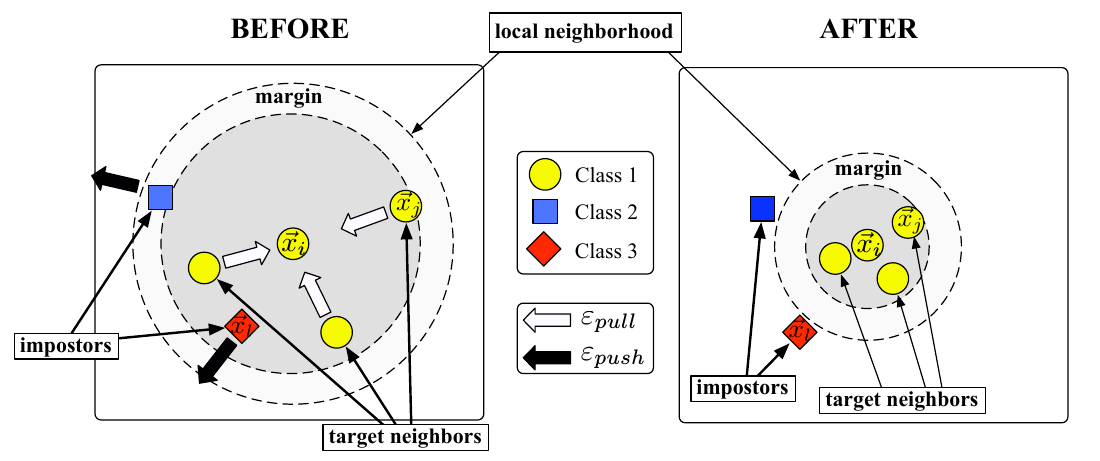
\includegraphics[width=5in, height=1.8in]{concepts/figures/metric_learning_example.png}
    \caption{Pictorial representation of metric learning and transformed space. Left image shows the
    representation of samples belonging to different classes. Right image shows the transformed space 
    from the learnt parameters. Notice that the samples from same class are moved closer to each other 
    and are pushed away from other class samples. Figure reference: Weinberger \etal ~\cite{weinberger07metric}.}
    \label{fig:metric_learning_example}
\end{figure}

Type of metric used to measure distance between two points in KNN algorithm plays an important role 
in determining its performance. If no prior knowledge of the data is available, KNN algorithm
is generally used with Euclidean distance measure. Since Euclidean metric does not hold any
statistical measure of data with respect to labels, it would lead to sub-optimal solutions. Methods such as
~\cite{Chopra:2005:LSM:1068507.1068961}, ~\cite{NIPS2004_2566}, ~\cite{Shalev-Shwartz:2004:OBL:1015330.1015376}, 
~\cite{Shental:2002:ALR:645318.649268} show that the performance of KNN improves by 
learning an appropriate distance metric. For example, distance metric learnt for face recognition
task and the gender detection task would be significantly different.

Consider $x = [x_1, x_2, \cdots , x_n]$ and $y = [y_1, y_2, \cdots , y_n]$ as two points in a $n$ dimensional space. The Euclidean distance, $d$ between these two points is
defined as

\begin{equation}
    d = \sqrt{(x_1-y_1)^2 + (x_2-y_2)^2 + . . . + (x_n-y_n)^2} 
\end{equation}

Even simple linear transformation learnt in supervised manner can lead to better performance in KNN 
classification as shown by ~\cite{Shalev-Shwartz:2004:OBL:1015330.1015376} and ~\cite{NIPS2004_2566}.
Consider a linear transformation matrix, $L$ which satisfies pseudo-metric properties such as triangular 
inequality, non-negativity, symmetry and uniqueness. The distance measured in the transformed space 
can be represented by,

\begin{equation}
    d_L = || L(x - y) ||^2
\end{equation}

The generalization of Euclidean metric is the Mahalanobis metric. The Mahalanobis distance between two
vectors is defined as,

\begin{equation}
    d_M = \sqrt{ (x-y)^T M (x-y) }
\end{equation}

\noindent
Where $M$ is a positive semi-definite matrix. Euclidean metric is a special case with $M = I$.

In this thesis (refer~\ref{subsec:euc_vs_metric}), we use metric to define degree of dissimilarity and also as probability. 
The vector under consideration for our approaches are to deal with the appearance of key feature on
the face or structural representation of the key features on the face. Clearly there is some
statistical information embedded across various points derived from these features. For example,
we could see significant correlation within the points representing an eye corner or a nose tip.
Also correlation is different when comparing between the eye corner and nose tip points. We
would like to use these statistical information residing in the labeled data to derive a 
suitable distance metric to improve the accuracy of our KNN based algorithm.

More specifically we use \textit{large margin nearest neighbor} (LMNN) classification algorithm~\cite{weinberger09distance}
to learn a Mahalanobis metric specifically designed for KNN classification. LMNN works on the 
intuitive idea that the test sample would be classified correctly if it lies near to samples of
same label. LMNN learns a linear transformation by minimizing a loss function that consists of 
two terms, where first term ensures the samples matching the labels are pulled together and 
second term pushes the samples with non-matching labels with large margin. Pictorially, it can
be represented as in Figure~\ref{fig:metric_learning_example}

% One can learn the parameters in Matrix M with M constrained to be a positive-semidefinite matrix to
% guarantee positive distances between any two points.
% 
% In our experiments, we consider modified version Nearest Neighbour called Large Margin Nearest Neighbour(LMNN).
% This algorithm was specifically designed to work well with KNN.
